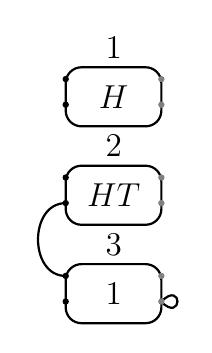
\begin{tikzpicture}[scale=0.5]
% The gate graph G 
\draw[thick,looseness=1.3] (0,-1.95cm) to [out=180,in=180] (0,-3.8cm);
\draw[thick,looseness = 200] (2.43,-4.45) to [out = 45, in = -45] (2.42,-4.45);  
 \foreach \offset/\unitary/\label in {0/H/1,-2.5/HT/2,-5/1/3}
{   
\begin{scope}[yshift=\offset cm]       
\draw[rounded corners=2mm,thick] (0,0) rectangle (2.43cm,1.5 cm);  
  \foreach \x /\color in {0/black,2.43/gray}
{     \foreach \y in {1.2,.55}
{       \draw[fill=\color,draw=\color] (\x cm, \y cm) circle (.66mm);
    }} 
  \node at (1.22cm, .75cm) {\large{$\unitary$}};   
 \node at (1.22cm, 2cm){\large{$\label$}};   
\end{scope}}  
\end{tikzpicture}